\documentclass{article}

% Language setting
% Replace `english' with e.g. `spanish' to change the document language
\usepackage[english]{babel}

% Set page size and margins
% Replace `letterpaper' with `a4paper' for UK/EU standard size
\usepackage[a4paper,top=2cm,bottom=2cm,left=3cm,right=3cm,marginparwidth=1.75cm]{geometry}

\usepackage{chngcntr}

\counterwithin*{section}{part} % Resets section counter after every part
\renewcommand{\thesection}{Ex \arabic{section}.} % Prefixing section numbers with "Ex"
\setcounter{section}{-1} % Starting section count from -1 so that it begins with "Ex 0."

% Useful packages
\usepackage{amsmath}
\usepackage{graphicx}
\usepackage[colorlinks=true, allcolors=blue]{hyperref}

\usepackage[product-units = power]{siunitx}
\sisetup{round-precision=2, separate-uncertainty = true, detect-weight=true, detect-family=true}
\usepackage[capitalise,nameinlink]{cleveref}
\usepackage{physics}
\AtBeginDocument{\RenewCommandCopy\qty\SI}
\usepackage[version=4]{mhchem}

\usepackage{booktabs}
\usepackage{multirow}

\title{MP2\\Path Integration using Coupled Bump Attractors\\---\\Computational neurosciences: neuronal dynamics\\NX-465}
\author{Konstantin Weindel}

\begin{document}
\maketitle


\section*{Introduction}
In this mini project 

\section{Getting Started: Poisson neurons}
\subsection*{0.1.}
\begin{figure}[h]
    \centering
    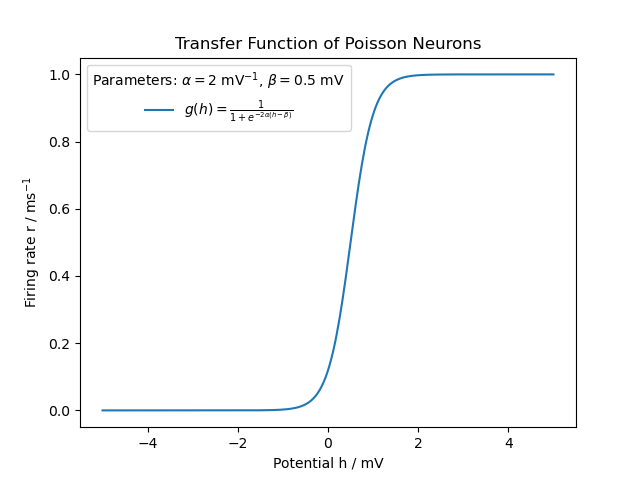
\includegraphics[width=0.7\textwidth]{figures/0.1.transfer_function.png}
    \caption{For Poisson Neurons, firing rate \(r\) in dependence of the potential \(h\) is described by a sigmoid function with parameters \(\alpha\) and \(\beta\).}
    \label{fig:01}
\end{figure}

The firing rate \(r_i\) of a Poisson Neuron \(i\) in dependence of it's potential \(h_i\) can be described by the in \cref{fig:01} depicted transfer function:
\[g(h_i(t)) = \frac{1}{1+\exp{-2\alpha(h_i(t)-\beta)}}.\]
The parameter $\alpha$ determines the steepness of the curve. A higher value of $\alpha$ makes the transition from the low firing rate to the high firing rate more abrupt.
The parameter $\beta$ sets the threshold potential at which the firing rate increases significantly. If $h_i(t)$ is much less than $\beta$, the firing rate $r_i(t)$ will be close to 0. If $h_i(t)$ is much greater than $\beta$, the firing rate will approach $r_0$.

\subsection*{0.2.}
\begin{table}[h]
\centering
\begin{tabular}{@{}rcc@{}}
\toprule
N    & mean number of spikes / \unit{\per\milli\second} & instantaneous rate r / \unit{\per\milli\second} \\ \midrule
100  &0.1173099& \multirow{2}{*}{0.1192043}                                                                                    \\
1000 &0.118458&                                                                                                               \\ \bottomrule
\end{tabular}
\caption{The number of spikes for a set of \(N\) neurons are calculated stochastically and analytically.}
\label{tab:02}
\end{table}

\Cref{tab:02} shows the result of the firing dynamics of unconnected neurons.
The mean number of spikes per ms across the N neurons differs from the instantaneous rate due to the stochastic nature of spike generation in the Poisson process. The actual spike count can vary around the expected value given by the rate equation.
With a larger number of neurons, the law of large numbers suggests that the mean spike count should more closely approximate the expected rate (instantaneous rate), reducing the variability seen in the smaller population.

\section{Bump attractor}
\subsection*{1.1.}
\begin{figure}[h!]
  \centering
  \begin{subfigure}[b]{0.32\textwidth}
    \includegraphics[width=\textwidth]{image1.png}
    \caption{First subplot}
    \label{fig:sub1}
  \end{subfigure}
  \hfill
  \begin{subfigure}[b]{0.32\textwidth}
    \includegraphics[width=\textwidth]{image2.png}
    \caption{Second subplot}
    \label{fig:sub2}
  \end{subfigure}
  \hfill
  \begin{subfigure}[b]{0.32\textwidth}
    \includegraphics[width=\textwidth]{image3.png}
    \caption{Third subplot}
    \label{fig:sub3}
  \end{subfigure}
  \caption{Three subplots side by side}
  \label{fig:test}
\end{figure}

For \(N=300\) neurons

\section{Integration}

\section{Path integration}


\end{document}